\documentclass[landscape,twocolumn,a4paper]{article}
\usepackage[utf8x]{inputenc}
\usepackage[ngerman]{babel}
\usepackage{listings}
\usepackage{babel}

\usepackage[T1]{fontenc}
\usepackage{booktabs} % schöne Tabellen
\usepackage{graphicx}
\usepackage{csquotes} % Anführungszeichen
\usepackage{paralist} % kompakte Aufzählungen
\usepackage{amsmath,textcomp,tikz} %diverses
\usepackage{eso-pic} % Bilder im Hintergrund
\usepackage{mdframed} % Boxen
\usepackage{multirow}
\usepackage{amssymb}

\usepackage{mathtools}
\usepackage[top=20mm,left=10mm,right=10mm,bottom=10mm]{geometry}
\usepackage{fancyhdr}
\pagestyle{fancy}
\fancyhead[L]{Beweise}
\fancyhead[R]{\thepage}
\fancyfoot{}

\lstset{language=Python, tabsize=4, basicstyle=\footnotesize, showstringspaces=false, mathescape=true}
\lstset{literate=%
  {Ö}{{\"O}}1
  {Ä}{{\"A}}1
  {Ü}{{\"U}}1
  {ß}{{\ss}}1
  {ü}{{\"u}}1
  {ä}{{\"a}}1
  {ö}{{\"o}}1
}
\begin{document}

\parindent 0mm


\textbf{Aufgaben der Zertifikatsklausuren}
\bigskip 

\textbf{A2020} \\
Es sei $f: (0,\infty) \rightarrow \mathbb{R}$ eine Funktion mit der Eigenschaft \\
(*) \quad $f(x\cdot y) = f(x) + f(y)$ für alle $x,y > 0$. \\
a) Beweisen Sie mit vollständiger Induktion, dass $f(2^n) = n \cdot f(2)$ für $n \in \mathbb{N}$ gilt. \\
b) Beweisen Sie, dass $f(1) = 0$ gilt. \\
c) Beweisen Sie, dass $f(\frac{1}{x}) = -f(x)$ für alle $x > 0$ gilt. \\

\textit{Hinweise:} Setzen Sie geeignete Werte für $x,y$ in (*) ein. Im Aufgabenteil c) darf das Ergebnis aus b)
verwendet werden, auch wenn Teil b) nicht gelöst wurde.
\bigskip

\textbf{A2019} \\
Für $n \in \mathbb{N}$ und $x \in \mathbb{R}$ sei $p_n(x) = 1 - x^{2^n}$. \\
a) Beweisen Sie durch vollständige Induktion, dass \\
$p_n(x) = (1-x)(1+x)(1+x^2)(1+x^4)...(1+x^{2^{n-1}})$ für alle $n \in \mathbb{N}$ mit $n \ge 2$ gilt. \\
b) Folgern Sie aus a), dass $p_n$ außer $x = \pm 1$ keine weiteren Nullstellen besitzt ($n \in \mathbb{N})$.
\bigskip

\textbf{A2018} \\
a) Gegeben sind vier positive reelle Zahlen $a_1, a_2, b_1, b_2 > 0$ mit der Eigenschaft
$\dfrac{a_1}{b_1} \le \dfrac{a_2}{b_2}$. Beweisen Sie, dass dann 
$\dfrac{a_1}{b_1} \le \dfrac{a_1+a_2}{b_1+b_2} \le \dfrac{a_2}{b_2}$ gilt. \\
b) Gegeben sind $2n$ positive Zahlen  $a_1, a_2,...,a_n b_1, b_2,...,b_n > 0$ mit der Eigenschaft \\
$\dfrac{a_1}{b_1} \le \dfrac{a_2}{b_2} ... \le \dfrac{a_{n-1}}{b_{n-1}} \le \dfrac{a_n}{b_n}$. \\
 Beweisen Sie, dass  
$\dfrac{a_1}{b_1} \le \dfrac{a_1+a_2+...+a_n}{b_1+b_2+...+b_n} \le \dfrac{a_n}{b_n}$ 
\bigskip

\newpage

\textbf{A2017} \\
Es sei $n \in \mathbb{N}$ mit $n \ge 3$. Ein einfaches n-Eck hat n verschiedene Eckpunkte $E_1,...,E_n$, die
durch Kanten verbunden sind. Außerdem schneiden sich die Kanten nicht, und für die Innenwinkel 
$\alpha_1,...,\alpha_n$ an den Ecken gilt: $\alpha_j \neq 0^\circ, 180^\circ, 360^\circ$ für $j=1,...,n$. \\
Beweisen Sie durch vollständige Induktion, dass für die Summe $S_n$ der Innenwinkel in einem einfachen
n-Eck mit $n \ge 3$ gilt: $S_n = (n-2) \cdot 180^\circ$. Hierbei darf ohne Beweis verwendet werden,
dass die Winkelsumme im Dreieck $180^\circ$ beträgt. \\
\textit{Hinweis:} Unterscheiden Sie im Induktionsschritt die Fälle $\alpha_{n+1} > 180^\circ$ und
$\alpha_{n+1} < 180^\circ$. Verwenden Sie die in der jeweiligen Skizze eingezeichnete Hilfslinie.

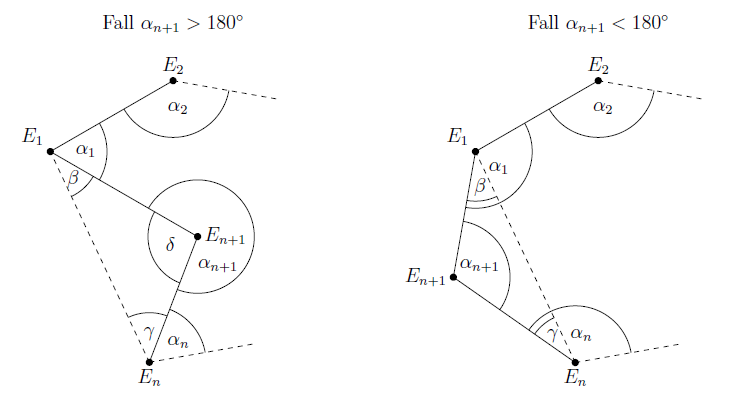
\includegraphics[scale=0.8]{bild2.png} \\
\bigskip

\newpage
\textbf{A2016} \\
In dieser Aufgabe beschäftigen wir uns mit den Sechseckszahlen $H_n (n=0,1,2,...)$. Wir betrachten
dazu Anordnungen von Kreisen mit gleichem Radius, die schrittweise folgendermaßen erzeugt werden:
Im Schritt 0 beginnen wir mit einem einzelnen Kreis, der im Schritt 1 wie unten skizziert durch
Anlagerung von sechs weiteren Kreisen zu einer sechseckartigen Figur ergänzt wird. Nachfolgend
wird im Schritt n + 1 die Figur aus dem Schritt n durch eine weitere äußere Lage von Kreisen zu
einer noch größeren sechseckartigen Figur ergänzt, wobei sich die Länge der äußeren Seiten um jeweils
eine Kugel erhöht. Die Sechseckzahl $H_n$ entspricht der Gesamtzahl der Kugeln in der so erzeugten
Figur im Schritt n. \\

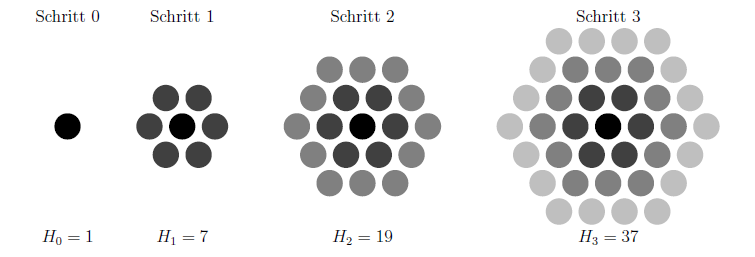
\includegraphics[scale=0.8]{bild1.png} \\

a) Drücken Sie $H_{n+1}$ durch $H_n$ aus $(n=0,1,2,...)$ \\
b) Zeigen Sie mit vollständiger Induktion, dass die n-te Sechseckzahl die Gleichung \\
 $H_n =3n^2 + 3n +1$ für 
$n \in \mathbb{N}$ erfüllt. \\
c) Zeigen Sie, dass die Summe der Sechseckzahlen gerade die Kubikzahlen
 $\sum\limits_{k=0}^{n-1} H_k = n^3$ liefert $n \in \mathbb{N}$. \textit{Hinweis:} Sie dürfen die Formel aus
 Teil b) verwenden, auch wenn Sie diese nicht bewiesen haben.
\bigskip

\newpage
\textbf{Sonstige Aufgaben}
\bigskip

\newcounter{y}
\setcounter {y} {1}


\textbf{A\arabic {y}:}
Eine Zahl $a \in \mathbb{R}$ heißt rational, wenn sie sich als Bruch $a = \frac{p}{q}$ mit ganzzahligen $p, q$ und 
$q \neq 0$ darstellen lässt. Gegeben seien eine feste rationale Zahl $a \neq 0$ und eine beliebige reelle Zahl $b$. Folgender Satz soll untersucht werden: Ist $b$ nicht rational, so ist auch $a \cdot b$ nicht rational.

a. Geben Sie Voraussetzung und Behauptung des Satzes an. \\
b. Bilden Sie die Kontraposition. \\
c. Beweisen Sie den Satz.
\bigskip \stepcounter{y}

\textbf{A\arabic {y}:}
Beweisen Sie mit vollständiger Induktion: Für alle natürlichen Zahlen gilt: \\

$\sum\limits_{k=1}^n (2k-1)^2 = \dfrac{n(2n+1)(2n-1)}{3}$
\bigskip \stepcounter{y}



\end{document}
